\documentclass[10pt,utf8]{beamer}

%\usepackage[utf8x]{inputenc}
\usepackage[ngerman]{babel}
\usepackage{amsmath}
\usepackage{bbm}

\usepackage{tabularx}
\usepackage{graphicx}
\usepackage{subfigure}
\usepackage{url}
%\usepackage{hyperref}
\usepackage{eurosym}
\usepackage{listings}

\usepackage{multirow}
\usepackage{colortbl}
\usepackage{booktabs}
\usepackage{setspace}
\usepackage{color, float}

\newif\ifzihbackground
\zihbackgroundtrue
%\zihbackgroundfalse

% Yes, this is dirty
\newcommand\zihmaketitle{
	\definecolor{white}{gray}{1.00}%
	\setbeamercolor{normaltext}{bg=darkblue}%
	\setbeamertemplate{headline}{%
		\vskip6.15mm\color{white}\setlength{\arrayrulewidth}{0.3pt}%
		\begin{tabular*}{\paperwidth}[b]{l@{\extracolsep\fill}}%
			\hspace*{3.0mm}\color{white}%
			
\includegraphics[height=7.81mm]{theme/logo/tu_logo_black}\\[1.2mm]%
			\hline\hspace*{11.76mm}\rule[-0.8mm]{0pt}{2.47mm}%
			\def\@@dummyComma{}\rule{0pt}{5.8pt}%
			\insertinstitute \\%
			\hline%
		\end{tabular*}%
		\hspace{-\paperwidth}%
	}%
    \ifzihbackground
      \setbeamertemplate{footline}{}
      \setbeamertemplate{background}{
\includegraphics[height=\paperheight,width=\paperwidth]{theme/logo/bg}}
      \else
      \setbeamertemplate{footline}{
          \parbox[t][22mm]{\paperwidth}{
              \vspace*{-8.18mm}
              \rule
              {98.6mm}{0pt}
\includegraphics[height=15mm]{theme/logo/zih_logo_white}

          }
      }
    \fi%
   \frame{\titlepage}
    % Kopf-/Fusszeilen fuer restliche Folien
    \setbeamercolor{normal text}{bg=white}
    \setbeamertemplate{background}{}
    \setbeamertemplate{headline}[zih01 theme]
    \setbeamertemplate{footline}[zih01 theme]
}

\usetheme{Dresden}
%\useoutertheme{theme/zih01}
%\useinnertheme{theme/zih01}
\usepackage{theme/beamerouterthemezih01}
\usepackage{theme/beamerinnerthemezih01}

%\useinnertheme{rounded}
\definecolor{darkblue}{rgb}{0.04, 0.16, 0.32}
% font color for headlines etc.
\setbeamercolor*{structure}{fg=darkblue,bg=white}
% disable navigation symbols
\setbeamertemplate{navigation symbols}{}
% can't remember what this is good for
\setbeamercovered{transparent}

% reduce margin size
\setbeamersize{text margin left=0.7cm}
\setbeamersize{text margin right=0.7cm}
%
% Outer Color Theme "whale" sorgt f?r strenge farbliche Trennen zwischen Zierrat
% und dem eigentlichen Inhalt. Ein dunkler Hintergrund f?r den Folientitel wirkt
% aber zu aufdringlich.
%
\usecolortheme{orchid}
%\setbeamercolor{titlelike}{parent=structure}

%
% Inner Color Theme "orchid" sorgt f?r farblich abgesetzt Bl?cke (Definitionen,
% S?tze, Beispiele, Beweise, ...).
%
%\usecolortheme{orchid}

%zum drucken
%\usepackage{pgfpages}
%\pgfpagesuselayout{resize to}[a4paper,border shrink=5mm,port]
%\pgfpagesuselayout{4 on 1}[a4paper,border shrink=3mm, landscape]

%%%%%%%%%%%%%%%%%%%%%%%%%%%%

\definecolor{LightGray}		{gray}{0.9}
\definecolor{Gray}		{gray}{0.5}
\definecolor{DarkGray}     	{gray}{0.2}
\definecolor{listinggray} 	{gray}{0.96}
\definecolor{DarkGreen}     	{rgb}{0.0,0.6,0.0}
\definecolor{DarkRed}     	{rgb}{0.6,0.0,0.0}
\definecolor{DarkBlue}     	{rgb}{0.0,0.0,0.6}
\definecolor{DarkCyan}     	{rgb}{0.7,0.7,0.2}
\definecolor{DarkDarkGreen}	{rgb}{0.0,0.4,0.0}

\lstset{language=C}
\lstset{linewidth=0.99\textwidth}
%\lstset{boxpos=c}
\lstset{xleftmargin=0.03\textwidth}
%\lstset{breaklines=true}
\lstset{framexleftmargin=0.03\textwidth}
\lstset{abovecaptionskip=\smallskipamount}
\lstset{belowcaptionskip=\smallskipamount}
\lstset{basicstyle=\ttfamily\tiny}
\lstset{backgroundcolor=\color{listinggray}}
%\lstset{frameround=ffff}
%\lstset{frame=shadowbox}
%\lstset{rulesepcolor=\color{Gray}}
\lstset{numbers=left}
\lstset{numberstyle=\tiny \color{DarkGray}}
\lstset{numbersep=0.01\textwidth}
\lstset{showstringspaces=false}
%\lstset{showspaces=false}
\lstset{tabsize=4}

%% all words in the following list are printed in bold letters in a listing 
\lstset{emph={__asm__, __volatile__, return, main,},emphstyle={\bfseries\color{DarkGray}}}
\lstset{captionpos=b}

% Style für C Sourcecode
\lstdefinestyle{CA}{
        language=C,
        basicstyle=\ttfamily\scriptsize,
        keywordstyle=\ttfamily\bfseries\color{DarkBlue},
        stringstyle=\ttfamily\color{DarkRed},
        commentstyle=\ttfamily\color{DarkGreen},
        identifierstyle=\ttfamily\color{DarkCyan},
        backgroundcolor=\color{listinggray},
}

%%%%%%%%%%%%%%%%%%%%%%%%%%%%

\title{Linux Cluster in Theorie und Praxis}
\subtitle{Mean Shift - parameterfreier Clusteringalgorithmus}
\author{Christian Deussen}
\date{4. M\"arz 2015}
\institute[ZIH TUD]{Zentrum f\"ur Informationsdienste und Hochleistungsrechnen -- TU Dresden}
%\room{INF 1046}
\address{N\"othnitzer Stra{\ss}e 46}
\city{01189 Dresden}
%\phone{+49 0351 - 463 38783}
\email{s3066193@mail.zih.tu-dresden.de}

\setbeamercovered{transparent}
\begin{document}

\zihmaketitle

\begin{frame}
\frametitle{Inhalt}
	\tableofcontents
\end{frame}
\Large

\section{Einführung}
\begin{frame}
	\frametitle{Einf\"uhrung}
		\centering
		\begin{figure}[p!]
			\vspace{-10pt}
			\hspace{-25pt}
			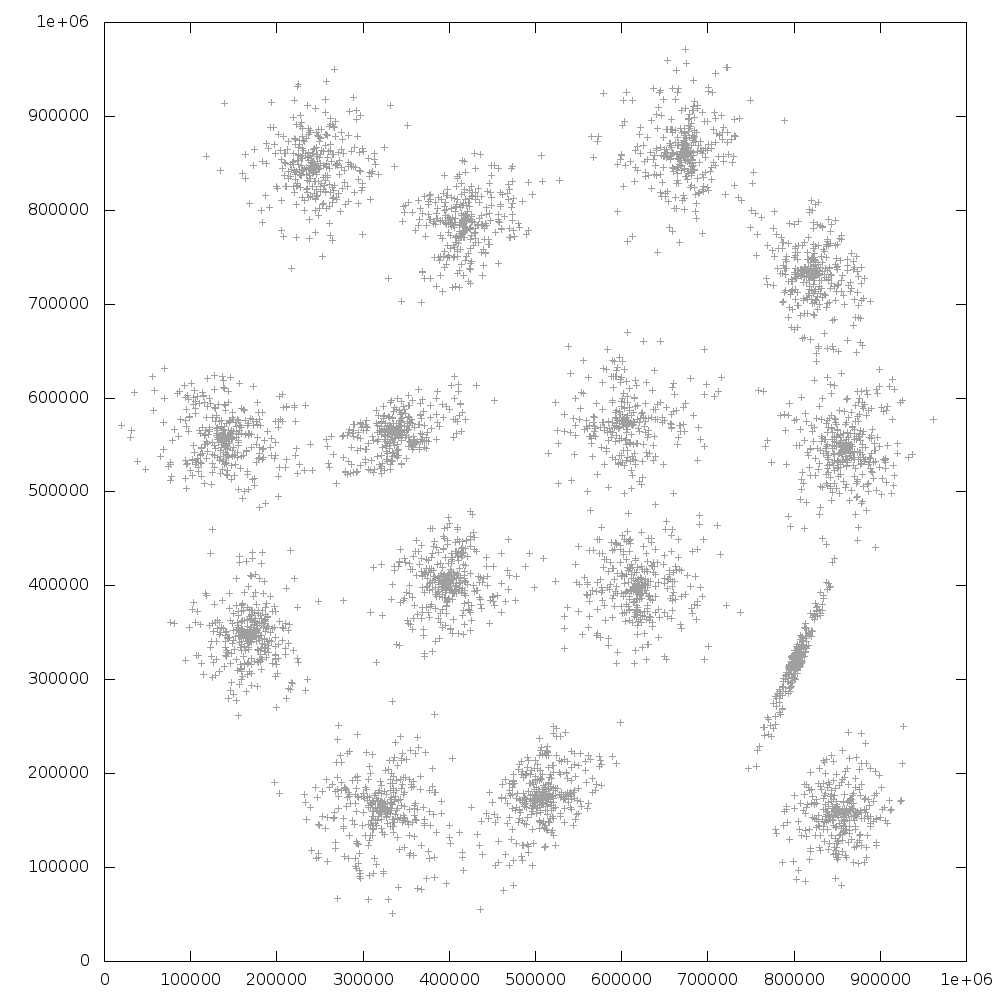
\includegraphics[scale=0.23, keepaspectratio]{../output/pics/s1_black.png}
			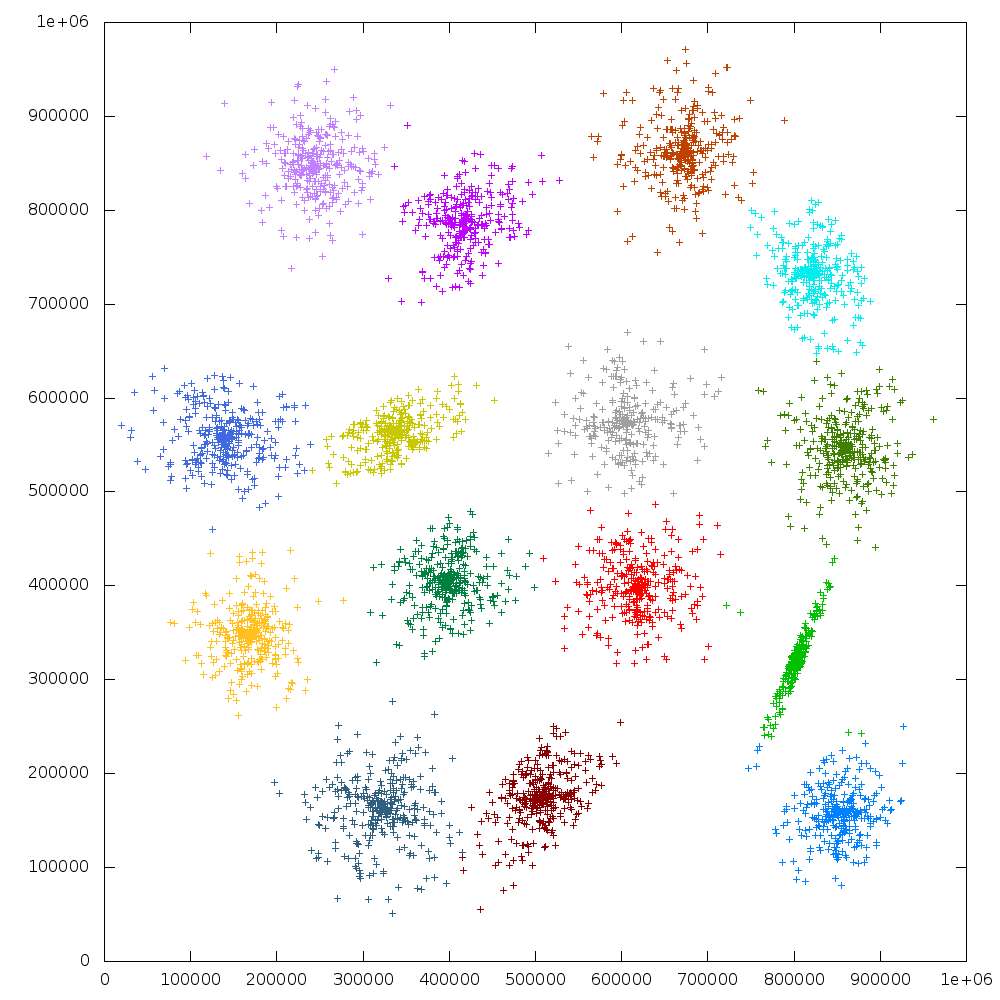
\includegraphics[scale=0.23, keepaspectratio]{../output/pics/s1_colored.png}
			\caption{Mean Shift Eingabe und Ausgabe [B0,B1]}
		\end{figure}
\end{frame}
\begin{frame}
	\frametitle{Einf\"uhrung}
\begin{figure}
	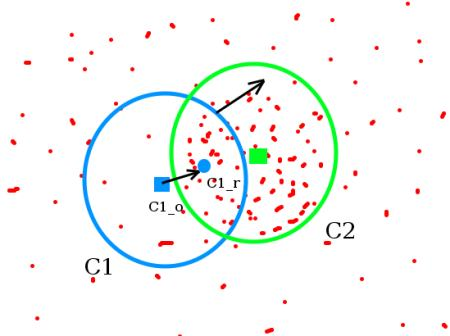
\includegraphics[scale=0.6]{meanshift_basics.jpg}
	\vspace{-10pt}
	\caption{Mean Shift Basics [B2]}
\end{figure}
\end{frame}
\begin{frame}
 		\[ m(x) = \frac{\sum_{x_i \in N(x)} K(x_i - x) x_i }{\sum_{x_i \in N(x)} K(x_i - x)} \]
\begin{figure}
    \begin{columns}%
        \begin{column}{0.5\textwidth}%
	  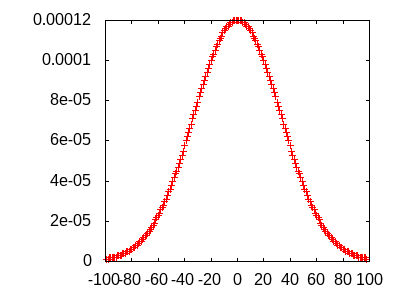
\includegraphics[scale=0.7]{../output/pics/gauss.png}
        \end{column}%
        \begin{column}{0.7\textwidth}%
			\vspace{-10pt}
			\hspace{35pt}
		\caption{Normierter Gaußkern [B3]}
        \end{column}%
    \end{columns}
\end{figure}
\end{frame}

\section{Implementation}
\begin{frame}[fragile]
	\frametitle{MPI Implementation}
	\begin{itemize}
		\item Einfach verkettete Liste
		\item Punkte werden statisch auf Cores gleichverteilt
	\end{itemize}
\normalsize
	\lstset{language=C,
		basicstyle=\ttfamily,
		keywordstyle=\color{blue}\ttfamily,
		stringstyle=\color{red}\ttfamily,
		commentstyle=\color{green}\ttfamily,
		morecomment=[l][\color{magenta}]{\#},
		numbers=none
        }
	\begin{lstlisting}
while(point) {
  if(point_cntr % numprocs == rank)
      point->cluster = meanshift(point->x, point->y);
  point = point->next;
  point_cntr++;
}
	\end{lstlisting}
\Large
	\begin{itemize}
		\item Hauptprozess führt Daten wieder zusammen
	\end{itemize}
\end{frame}
\begin{frame}
	\frametitle{MPI}
	\begin{itemize}
		\item Optimale Auslastung nicht sicher
		\item Keine Zwischenergebnisse
		\item wenig Kommunikation
		\item Genauigkeit von Gleitkommazahlen muss beachtet werden
	\end{itemize}
\end{frame}

\section{Beispiele}
\begin{frame}  
	\frametitle{Beispiel S2.txt}
	\begin{tabular}{cl}  
		\begin{tabular}{c}
			\vspace{-5pt}
			\hspace{-19pt}
			\parbox{0.5\linewidth}{%  change the parbox width as appropiate
				\begin{itemize}
					\item 5.000 Punkte
					\item 9 Minuten Laufzeit auf einem Core
					\item Kernelgröße 100.000
				\end{itemize}
			}
		\end{tabular}
		& \begin{tabular}{l}
			\vspace{-5pt}
			\hspace{-35pt}
			\parbox{0.5\linewidth}{%  change the parbox width as appropiate
				\begin{figure}
					\centering
					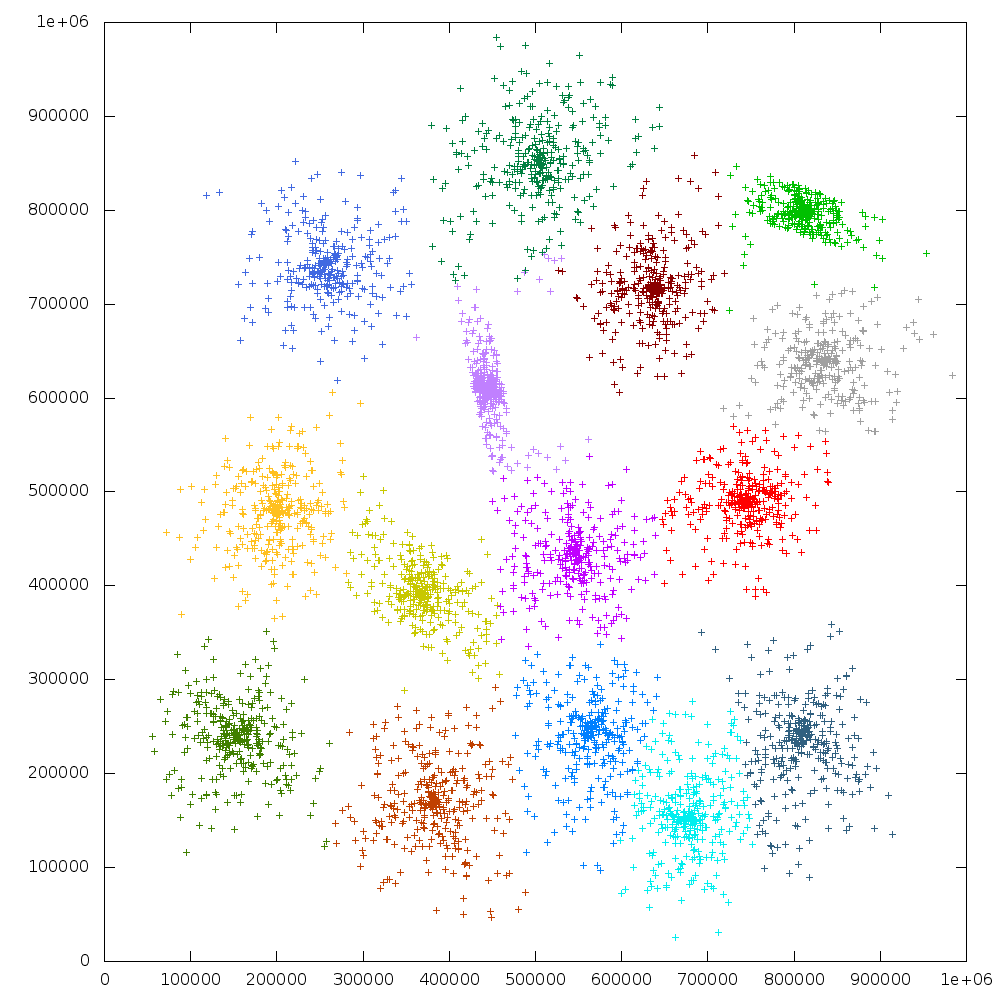
\includegraphics[scale=0.24, keepaspectratio]{../output/pics/s2_colored.png}
					\vspace{-5pt}
					\caption{S2 Colored [B4]}
				\end{figure}
			}
		\end{tabular}\\
	\end{tabular}
\end{frame}

\begin{frame}
	\hspace{-16pt}
	\begin{figure}
		\centering
		\vspace{-31pt}
		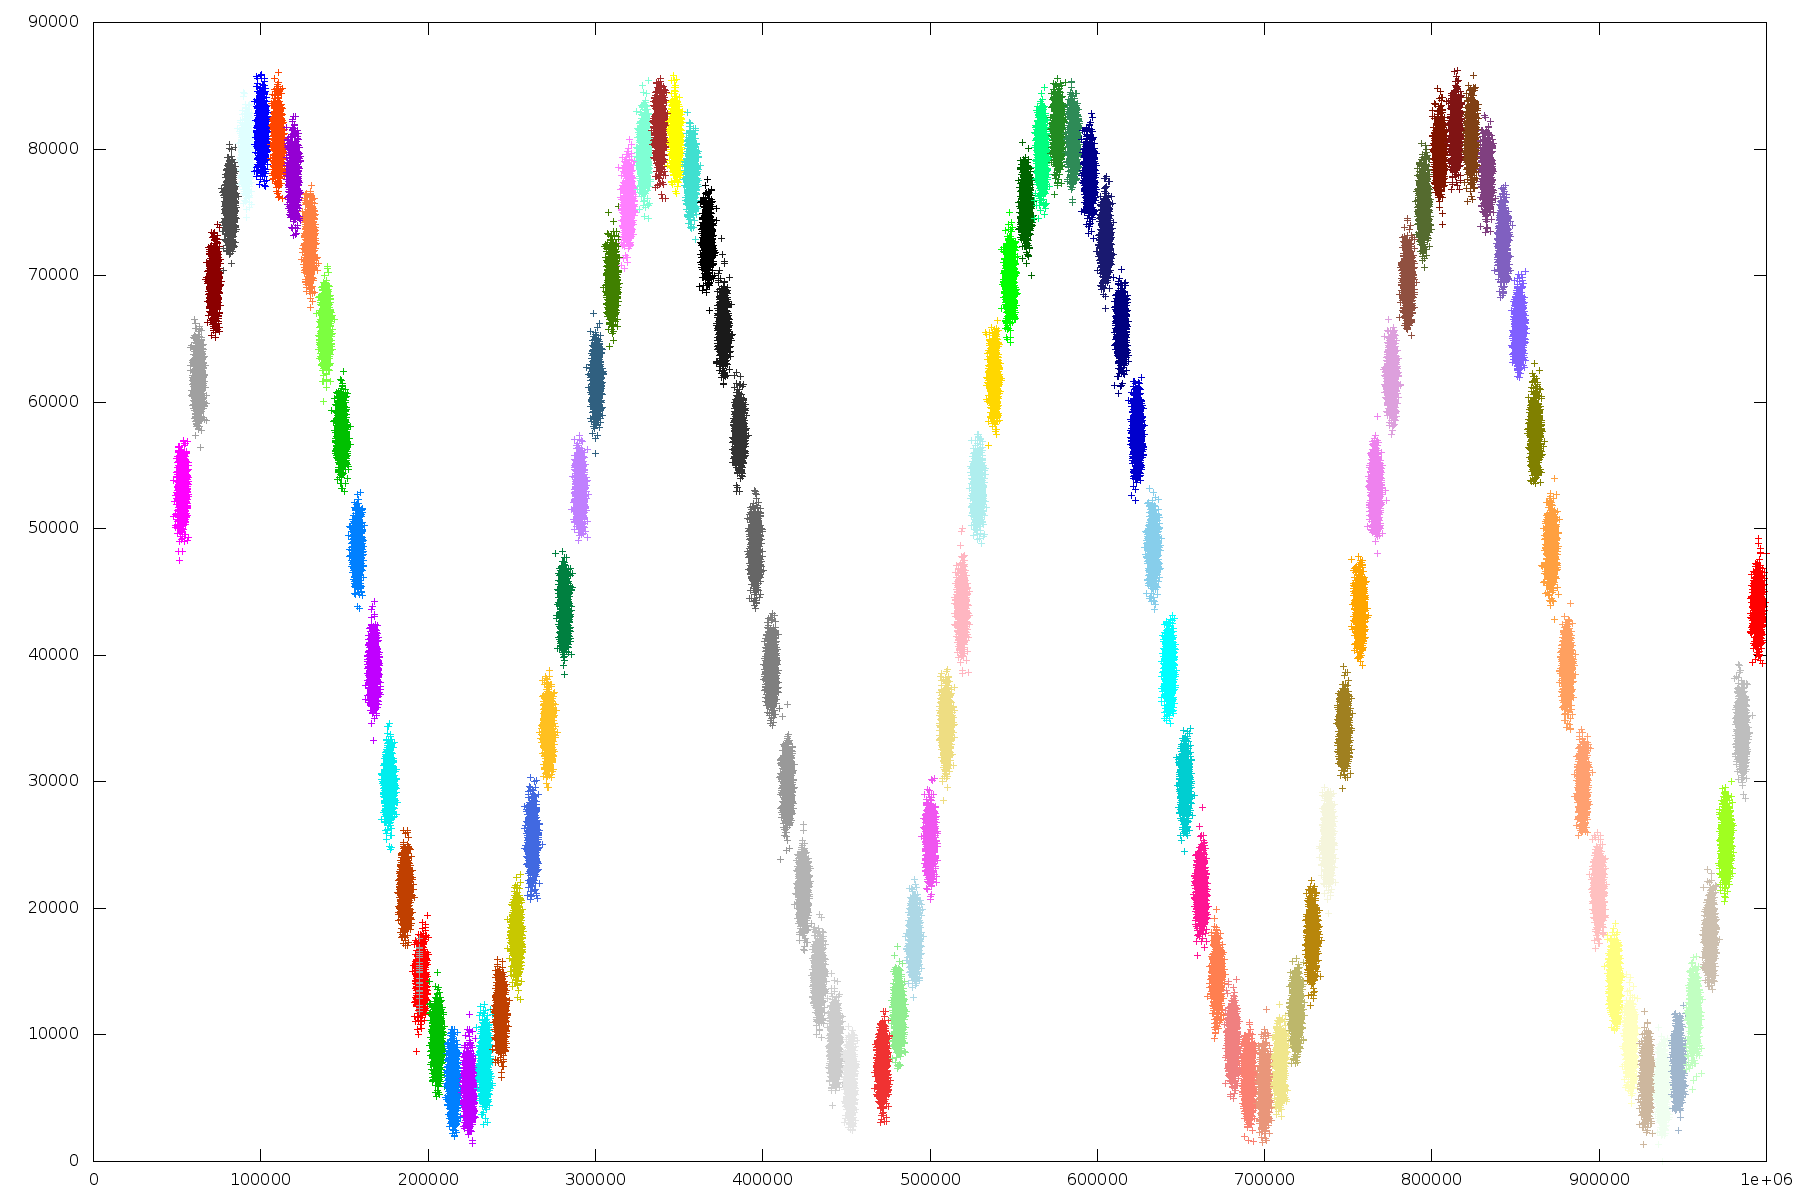
\includegraphics[scale=0.25, keepaspectratio]{../output/pics/sine.png} 
		\vspace{-14pt}
		\caption{Birch3 Colored [B5]}
	\end{figure}
	%nur 41 Sekunden Laufzeit auf 128 Cores
\end{frame}

\begin{frame}  
	\frametitle{Beispiel Birch3.txt}
	\begin{tabular}{cl}  
		\begin{tabular}{c}
			\vspace{-5pt}
			\hspace{-19pt}
			\parbox{0.5\linewidth}{%  change the parbox width as appropiate
				\begin{itemize}
					\item 100.000 Punkte
					\item 6 Minuten Laufzeit auf 128 Cores
					\item Kernelgröße 50.000
					\item Kleine Artefakte 
				\end{itemize}
			}
		\end{tabular}
		& \begin{tabular}{l}
			\vspace{-5pt}
			\hspace{-35pt}
			\parbox{0.5\linewidth}{%  change the parbox width as appropiate
				\begin{figure}
					\centering
					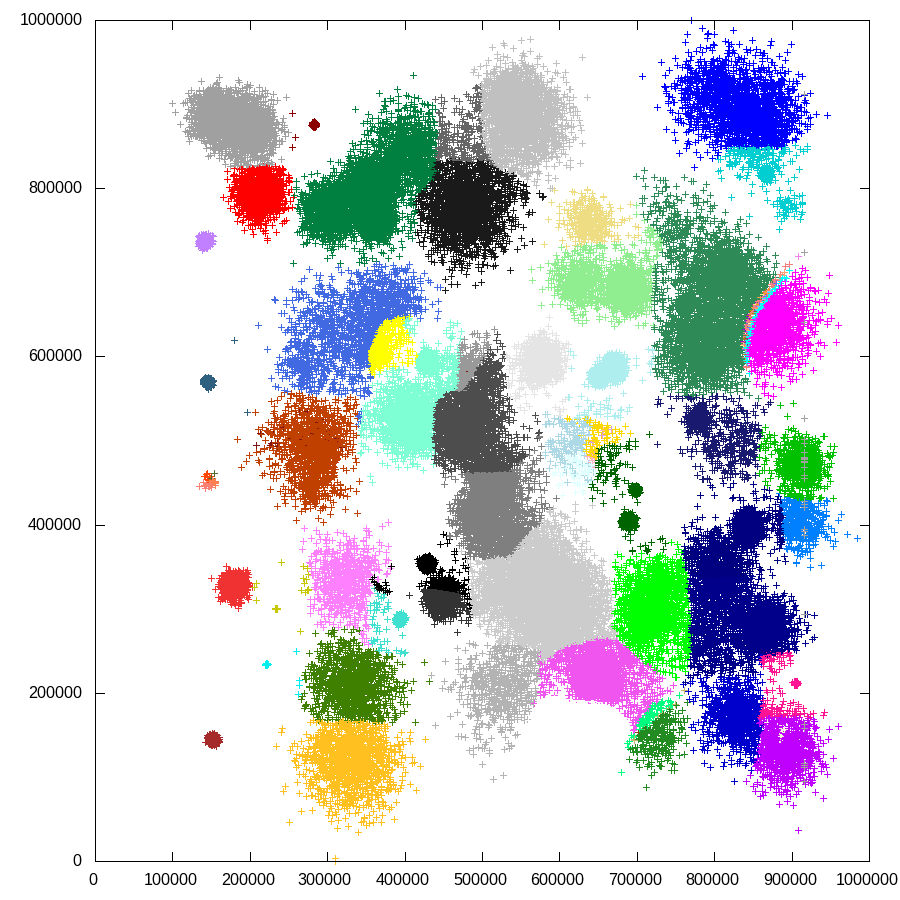
\includegraphics[scale=0.264, keepaspectratio]{../output/pics/birch3_colored.png}
					\vspace{-5pt}
					\caption{Birch3 Colored [B6]}
				\end{figure}
			}
		\end{tabular}\\
	\end{tabular}
\end{frame}
\begin{frame}
	\frametitle{Beispiele}
	\centering
	\begin{figure}[p!]
		\vspace{-10pt}
		\hspace{-25pt}
		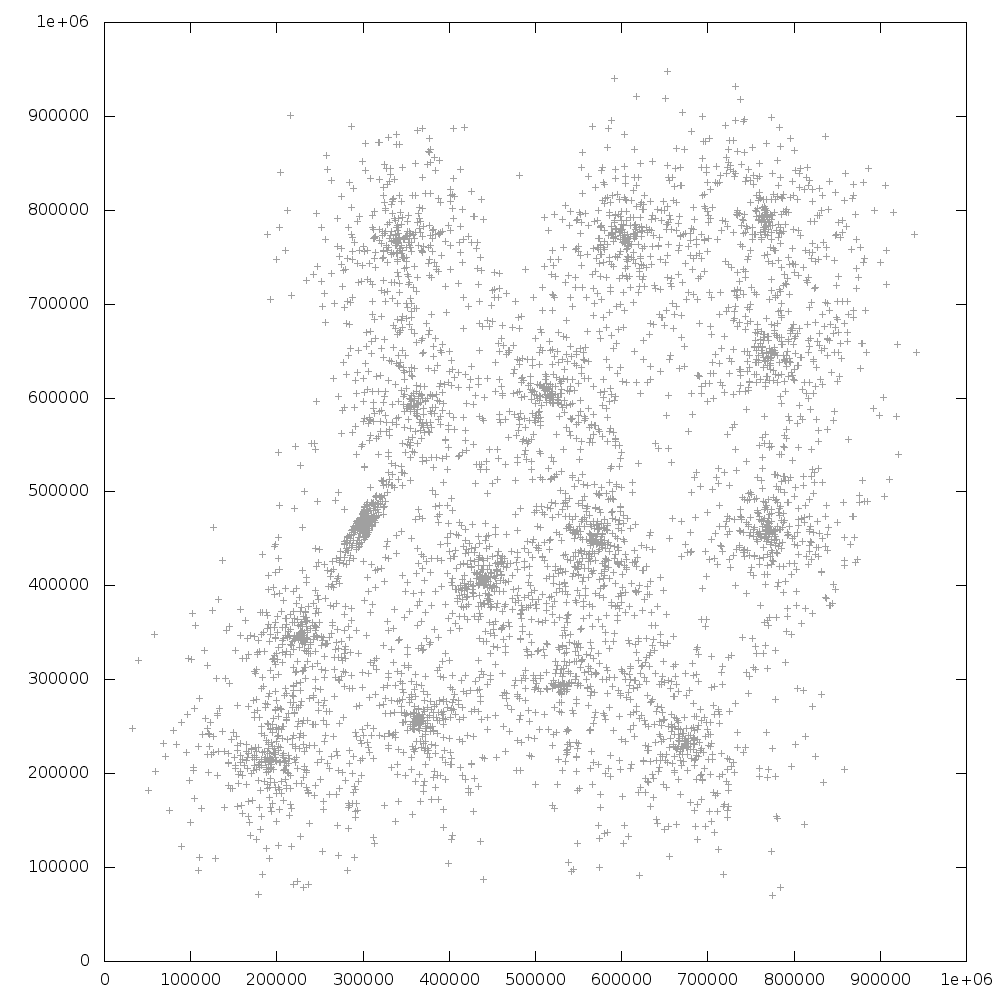
\includegraphics[scale=0.23, keepaspectratio]{../output/pics/s3_black.png}
		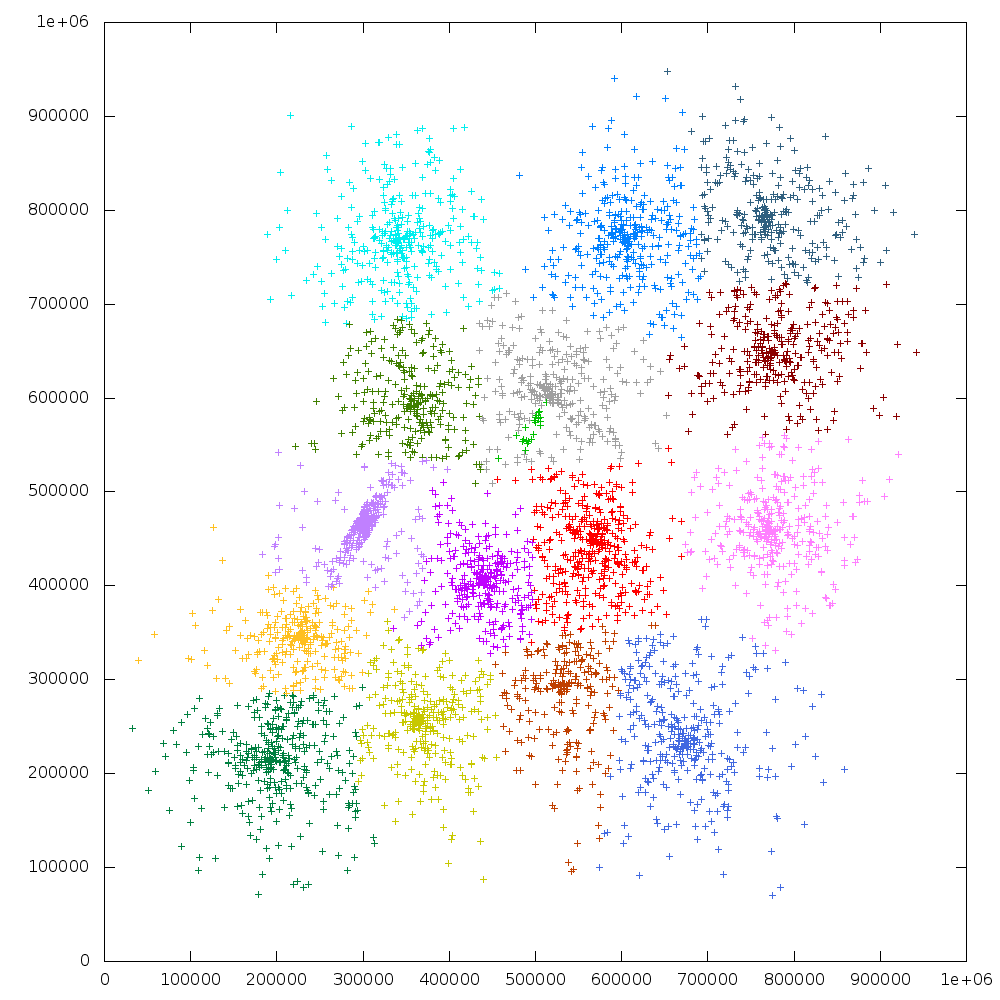
\includegraphics[scale=0.23, keepaspectratio]{../output/pics/s3_colored.png}
		\caption{Mean Shift Eingabe und Ausgabe [B7,B8]}
	\end{figure}
\end{frame}
\section{Benchmarks}
\begin{frame}  
	\frametitle{Cluster Benchmark}
	\begin{tabular}{cl}  
		\begin{tabular}{c}
			\vspace{-5pt}
			\hspace{-36pt}
			\parbox{0.5\linewidth}{%  change the parbox width as appropiate
				\begin{itemize}
					\item Taurus Node hat 2x8 Cores
					\item Ab 16 Cores Kommunikation über Netzwerk
				\end{itemize}
			}
		\end{tabular}
		& \begin{tabular}{l}
			\vspace{-15pt}
			\hspace{-49pt}
			\parbox{0.5\linewidth}{%  change the parbox width as appropiate
				\vspace{-15pt}
				\begin{figure}[H!]
					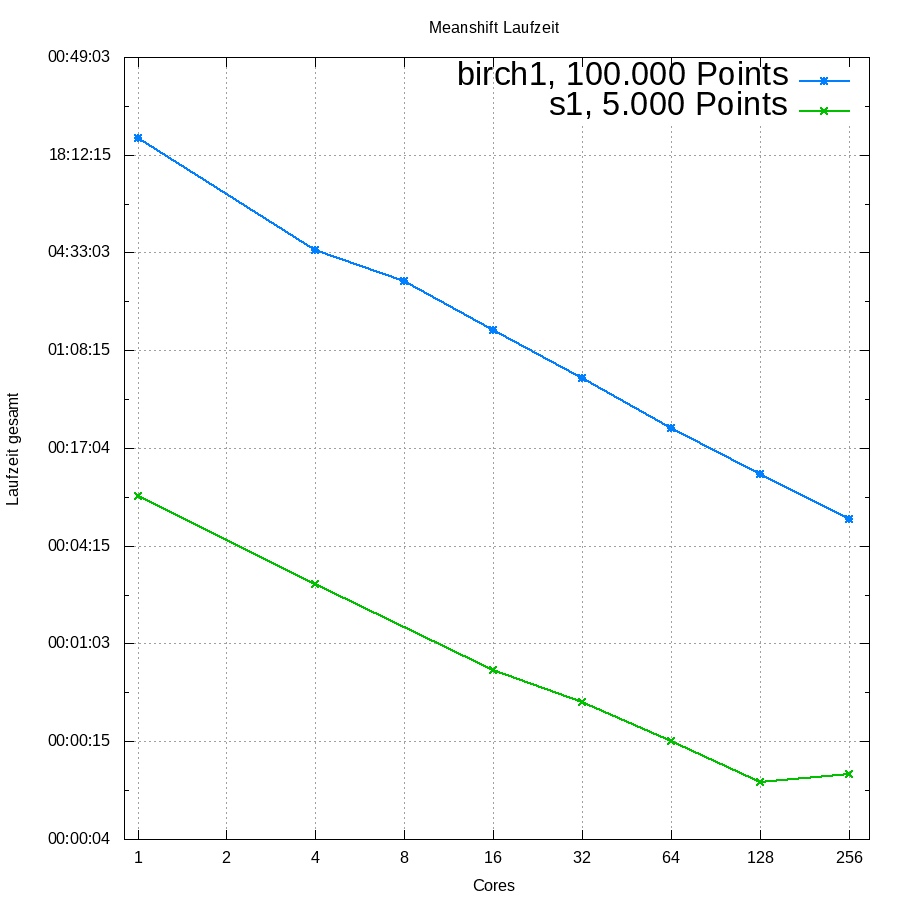
\includegraphics[scale=0.31, keepaspectratio]{../output/pics/benchmark.png}
					\vspace{-10pt}
					\caption{Laufzeit Benchmark [B9]}
				\end{figure}
			}
		\end{tabular}\\
	\end{tabular}
\end{frame}

\begin{frame}  
	\frametitle{Cluster Benchmark}
	\begin{tabular}{cl}  
		\begin{tabular}{c}
			\vspace{-5pt}
			\hspace{-36pt}
			\parbox{0.5\linewidth}{%  change the parbox width as appropiate
				\begin{itemize}
					\item Speedup nimmt bei vielen Cores ab
					\item Overhead bei kleinen Problemen groß
				\end{itemize}
			}
		\end{tabular}
		& \begin{tabular}{l}
			\vspace{-15pt}
			\hspace{-49pt}
			\parbox{0.5\linewidth}{%  change the parbox width as appropiate
				\vspace{-15pt}
				\begin{figure}[H!]
					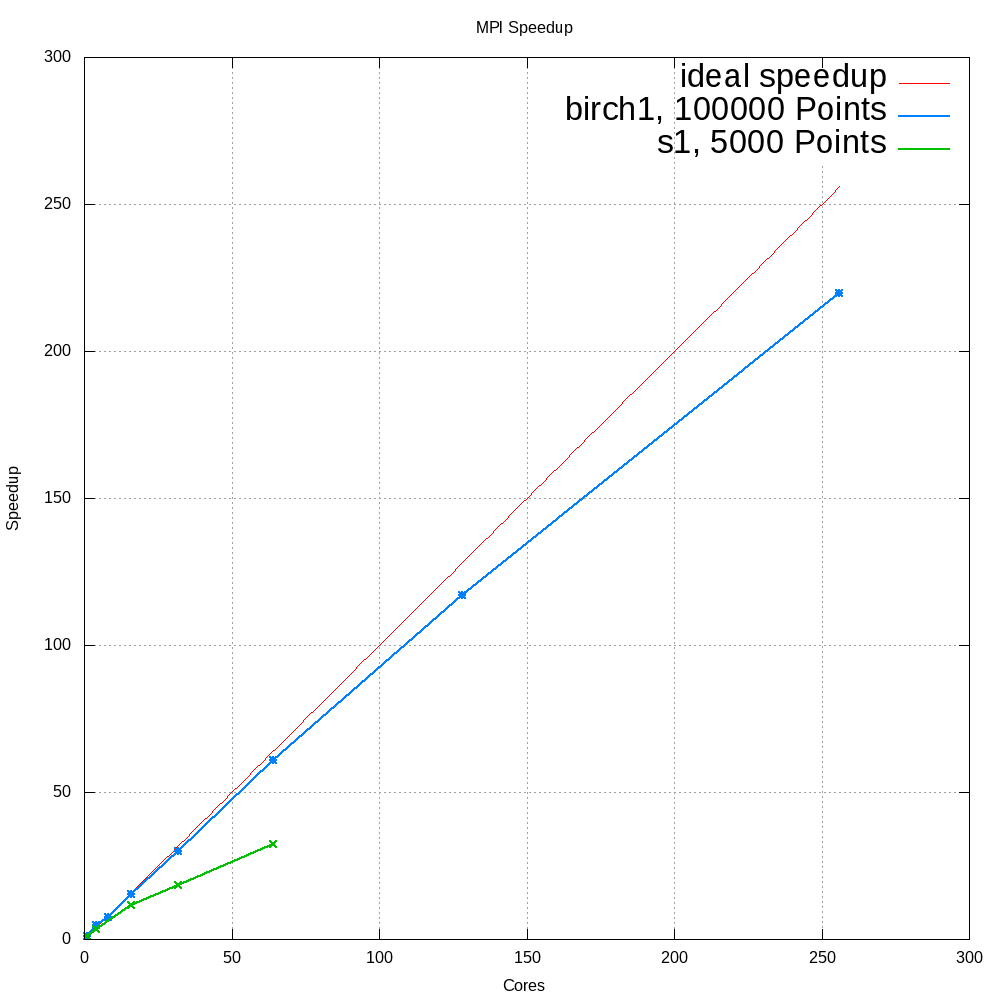
\includegraphics[scale=0.31, keepaspectratio]{../output/pics/speedup.png}
					\vspace{-10pt}
					\caption{Speedup [B10]}
				\end{figure}
			}
		\end{tabular}\\
		& \begin{tabular}{l}
			\vspace{-5pt}
			\hspace{-49pt}
		\end{tabular}\\
	\end{tabular}
\end{frame}

\begin{frame}
	\centering
	\begin{figure}[p!]
		\vspace{-10pt}
		\hspace{-25pt}
		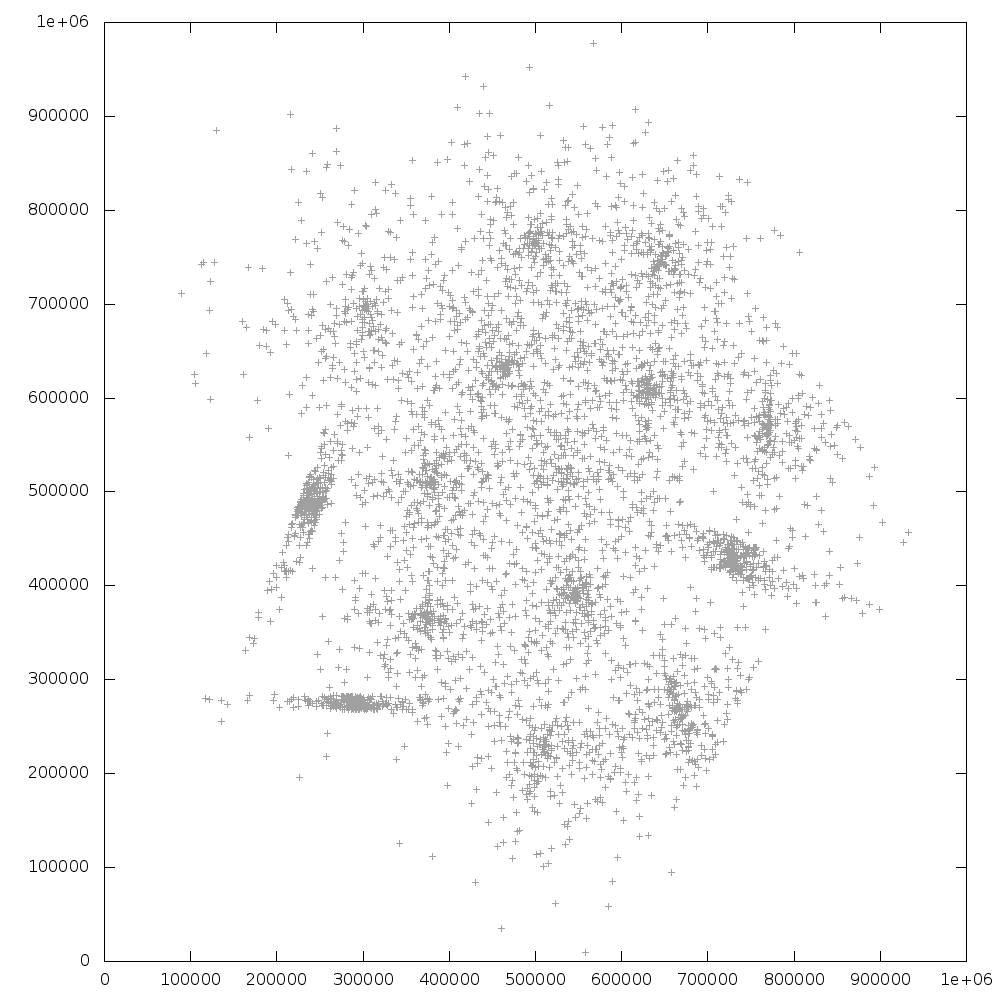
\includegraphics[scale=0.23, keepaspectratio]{../output/pics/s4_black.png}
		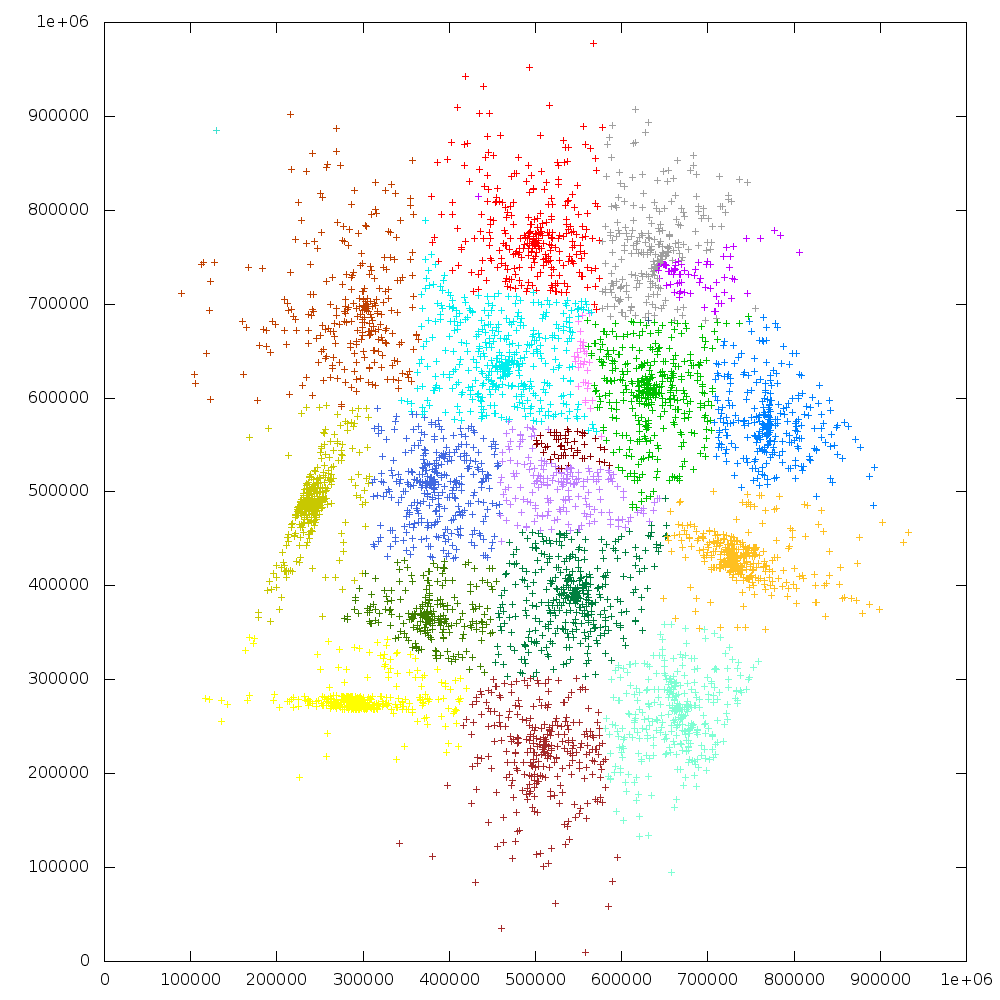
\includegraphics[scale=0.23, keepaspectratio]{../output/pics/s4_colored.png}
		\caption{Mean Shift Eingabe und Ausgabe [B11,B12]}
	\end{figure}
\end{frame}
\begin{frame}
\frametitle{Quellen}
\framesubtitle{}
\tiny
\subsection*{Textquellen}
	\begin{itemize}[]
		\bibitem [0] {} Mean Shift \url{http://homepages.inf.ed.ac.uk/rbf/CVonline/LOCAL_COPIES/TUZEL1/MeanShift.pdf}
		\bibitem [1] {} Mean Shift: Construction and Convergence Proof \url{http://www.cse.yorku.ca/~kosta/CompVis_Notes/mean_shift_derivation.pdf}
		\bibitem [2] {} Datasets \url{http://cs.joensuu.fi/sipu/datasets/}
		\bibitem [3] {} Taurus TU Dresden \url{https://doc.zih.tu-dresden.de/hpc-wiki/bin/view/Compendium/SystemTaurus}
		\bibitem [4] {} Mean Shift \url{https://courses.csail.mit.edu/6.869/handouts/PAMIMeanshift.pdf}
		\bibitem [B0] {} Mean Shift Basics \url{http://docs.opencv.org/trunk/_images/meanshift_basics.jpg}
	\end{itemize}
\end{frame}
\end{document}
